\documentclass{beamer}
\usepackage[english, russian]{babel}
\usepackage[T2A]{fontenc}
\usepackage[utf8]{inputenc}
\usepackage{indentfirst}
\usepackage{amsmath, amsfonts, amssymb, amsthm, mathtools}
\usepackage[export]{adjustbox}
\usepackage{graphicx} 
\graphicspath{ {./images/} }

\usepackage{subcaption}
\usepackage{verbatim}

\usepackage{minted}{\setlength{\parskip}{0pt}}

\usepackage{hyperref}

\hypersetup{
    colorlinks=true,
    linkcolor=blue,
    filecolor=magenta,      
    urlcolor=black,
    pdftitle={Overleaf Example},
    pdfpagemode=FullScreen,
    }


\title{Лабораторная работа № 13. \\ Настройка NFS}
\author{Данила Стариков \\ НПИбд-02-22}
\institute{Российский университет дружбы народов имени Патриса Лумумбы}
\date{2024}

\begin{document}

\frame{\titlepage}

\begin{frame}
\frametitle{Цель работы}
\begin{itemize}
    \item Приобретение навыков настройки сервера NFS для удалённого доступа к ресурсам.
\end{itemize}
\end{frame}

% section 1
\begin{frame}
\frametitle{Настройки сервера NFSv4}
    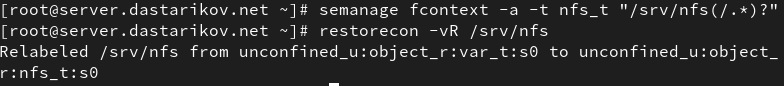
\includegraphics[width=\textwidth]{../images/image01.png}
    \captionof{figure}{Создание контекста безопасности для каталога /srv/nfs.}
\end{frame}


\begin{frame}
\frametitle{Настройки сервера NFSv4}
    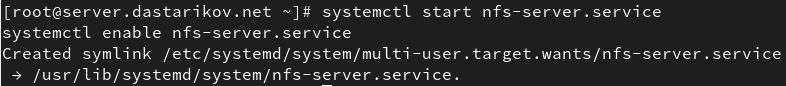
\includegraphics[width=\textwidth]{../images/image02.png}
    \captionof{figure}{Запуск сервера NFS.}
\end{frame}


\begin{frame}
\frametitle{Настройки сервера NFSv4}
    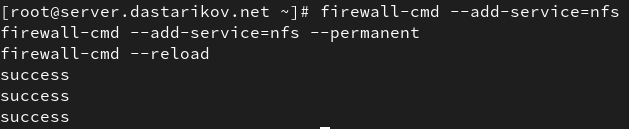
\includegraphics[width=\textwidth]{../images/image03.png}
    \captionof{figure}{Настройка межсетевого экрана.}
\end{frame}


\begin{frame}
\frametitle{Настройки сервера NFSv4}
    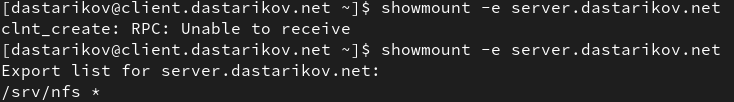
\includegraphics[width=\textwidth]{../images/image04.png}
    \captionof{figure}{Попытки подключения к удаленно смонтированному ресурсу.}
\end{frame}


\begin{frame}
\frametitle{Настройки сервера NFSv4}
    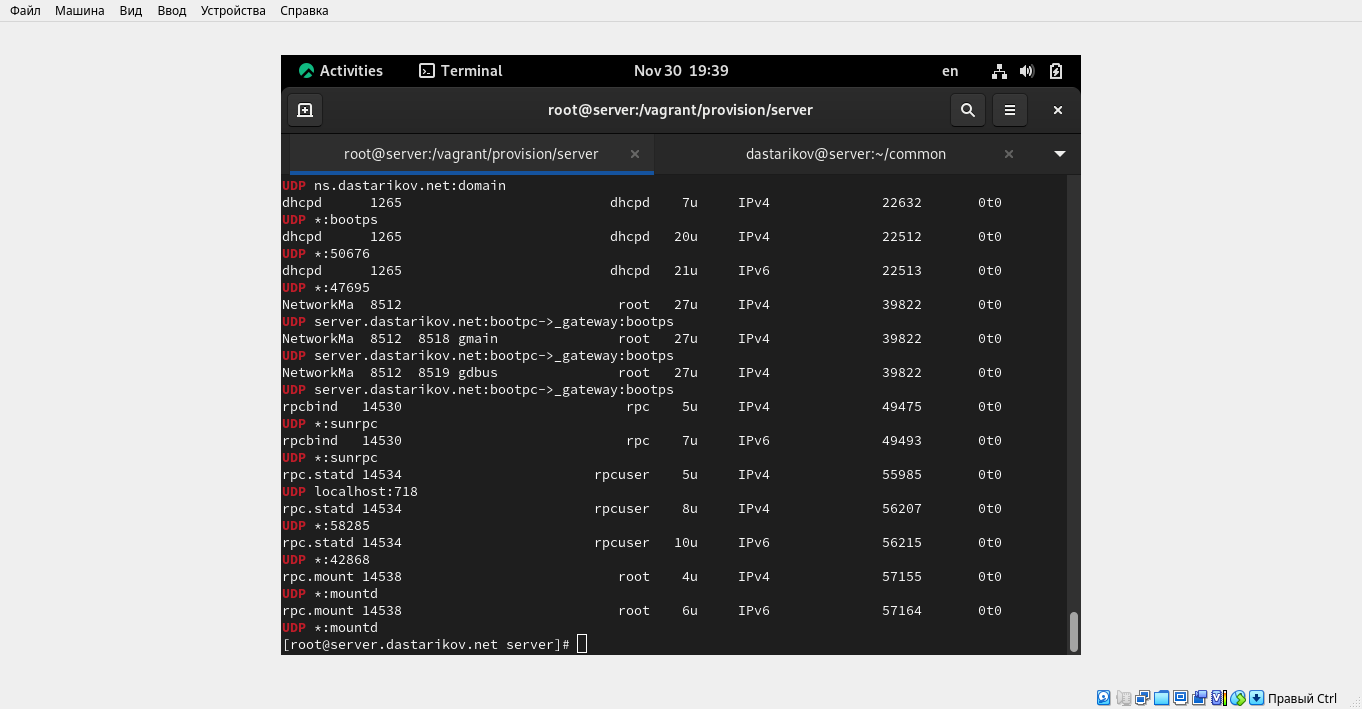
\includegraphics[width=\textwidth]{../images/image30.png}
    \captionof{figure}{Задействованные службы по протоколу UDP.}
\end{frame}


\begin{frame}
\frametitle{Настройки сервера NFSv4}
    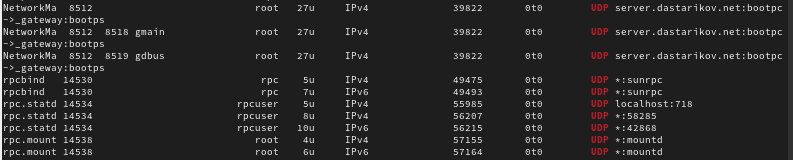
\includegraphics[width=\textwidth]{../images/image31.png}
    \captionof{figure}{Задействованные службы по протоколу TCP.}
\end{frame}


\begin{frame}
\frametitle{Настройки сервера NFSv4}
    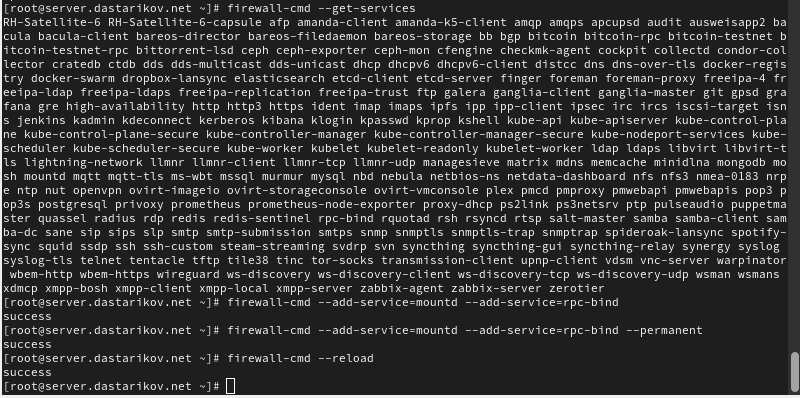
\includegraphics[width=\textwidth]{../images/image05.png}
    \captionof{figure}{Добавление служб rpc-bind и mountd в настройки межсетевого экрана.}
\end{frame}


\begin{frame}
\frametitle{Настройки сервера NFSv4}
    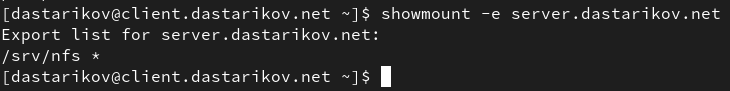
\includegraphics[width=\textwidth]{../images/image06.png}
    \captionof{figure}{Проверка подключения удаленного ресурса.}
\end{frame}

% section 2

\begin{frame}
\frametitle{Монтирование NFS на клиенте}
    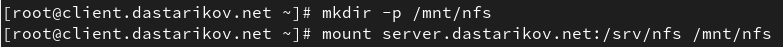
\includegraphics[width=\textwidth]{../images/image07.png}
    \captionof{figure}{Создание каталога на клиенте, в который будет монтироваться удаленный ресурс.}
\end{frame}

\begin{frame}
\frametitle{Монтирование NFS на клиенте}
    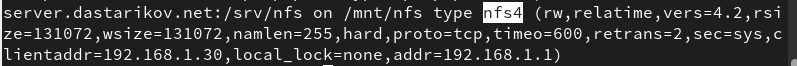
\includegraphics[width=\textwidth]{../images/image08.png}
    \captionof{figure}{Проверка правильности подключения ресурса NFS.}
\end{frame}

\begin{frame}
\frametitle{Монтирование NFS на клиенте}
    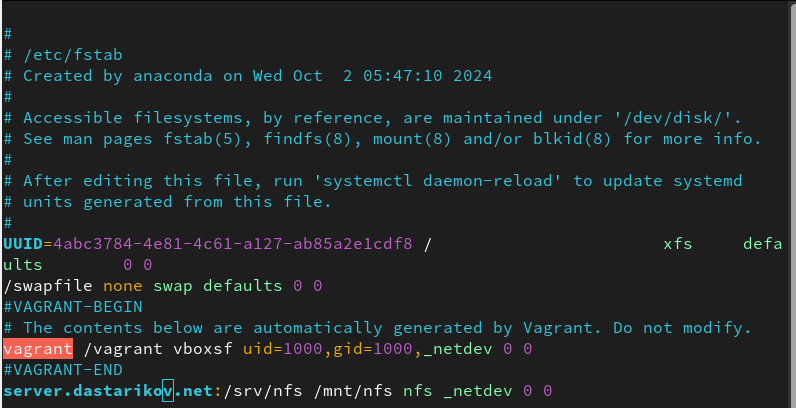
\includegraphics[width=\textwidth]{../images/image09.png}
    \captionof{figure}{Изменение файла /etc/fstab.}
\end{frame}

\begin{frame}
\frametitle{Монтирование NFS на клиенте}
    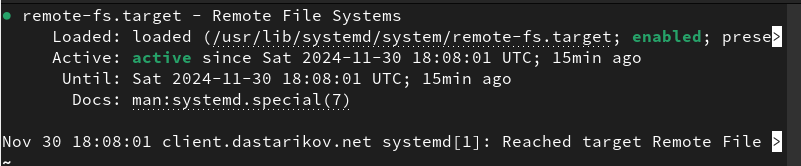
\includegraphics[width=\textwidth]{../images/image10.png}
    \captionof{figure}{Проверка автоматического монтирования удаленных ресурсов на клиенте.}
\end{frame}

\begin{frame}
\frametitle{Монтирование NFS на клиенте}
    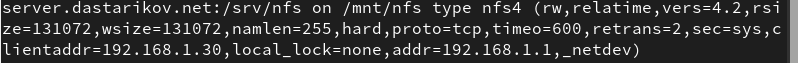
\includegraphics[width=\textwidth]{../images/image11.png}
    \captionof{figure}{Проверка автоматического монтирования после перезагрузки клиента.}
\end{frame}

% section 3

\begin{frame}
\frametitle{Подключение каталогов к дереву NFS}
    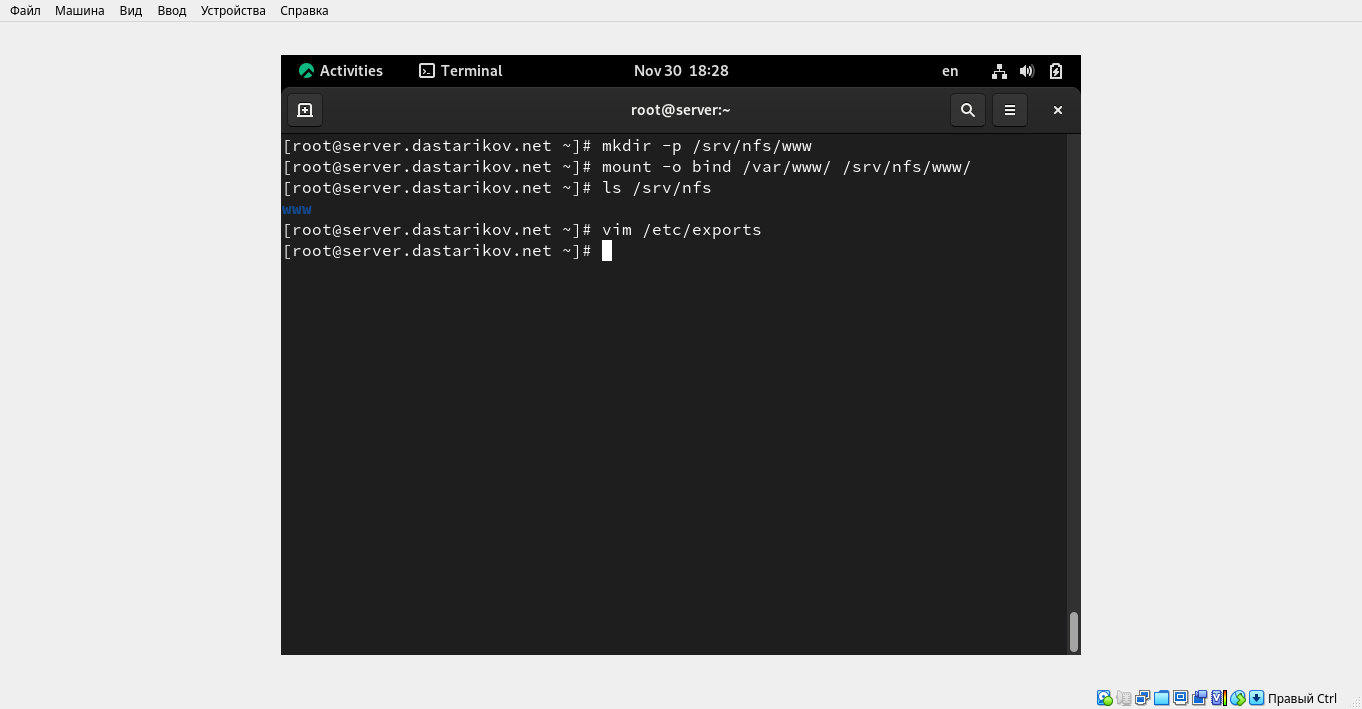
\includegraphics[width=\textwidth]{../images/image15.png}
    \captionof{figure}{Создание общего каталога с контентом веб-сервера.}
\end{frame}

\begin{frame}
\frametitle{Подключение каталогов к дереву NFS}
    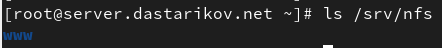
\includegraphics[width=\textwidth]{../images/image12.png}
    \captionof{figure}{Проверка содержимого /srv/nfs.}
\end{frame}

\begin{frame}
\frametitle{Подключение каталогов к дереву NFS}
    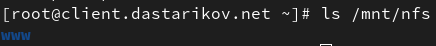
\includegraphics[width=\textwidth]{../images/image13.png}
    \captionof{figure}{Проверка содержимого /mnt/nfs.}
\end{frame}

\begin{frame}
\frametitle{Подключение каталогов к дереву NFS}
    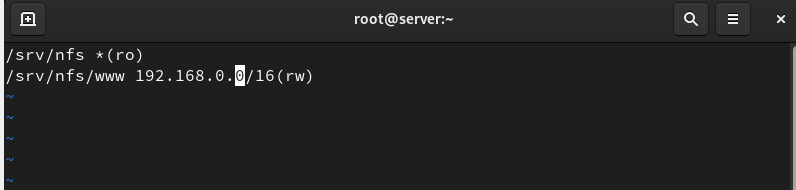
\includegraphics[width=\textwidth]{../images/image14.png}
    \captionof{figure}{Изменение файла /etc/exports.}
\end{frame}

\begin{frame}
\frametitle{Подключение каталогов к дереву NFS}
    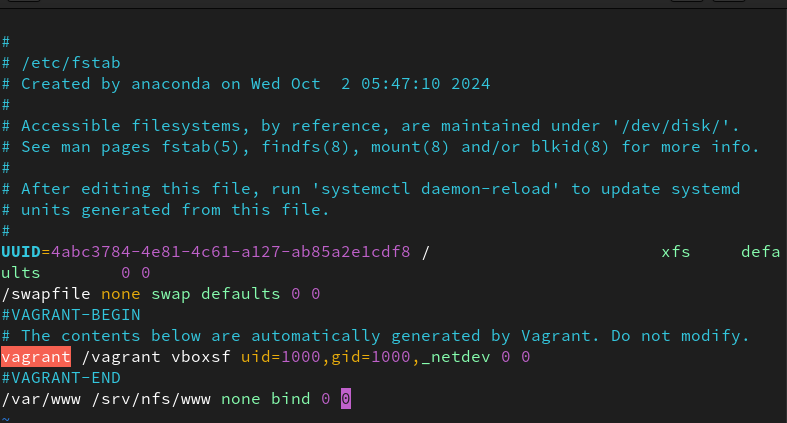
\includegraphics[width=\textwidth]{../images/image19.png}
    \captionof{figure}{Изменение файла /etc/fstab.}
\end{frame}

\begin{frame}
\frametitle{Подключение каталогов к дереву NFS}
    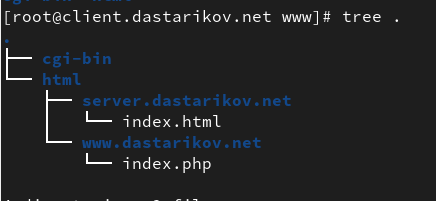
\includegraphics[width=\textwidth]{../images/image20.png}
    \captionof{figure}{Содержимое каталога /mnt/nfs/www.}
\end{frame}

% section 4

\begin{frame}
\frametitle{Подключение каталогов для работы пользователей}
    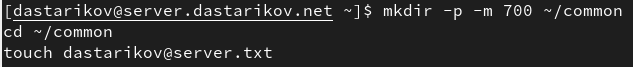
\includegraphics[width=\textwidth]{../images/image21.png}
    \captionof{figure}{Создание личного каталога common для пользователя dastarikov.}
\end{frame}

\begin{frame}
\frametitle{Подключение каталогов для работы пользователей}
    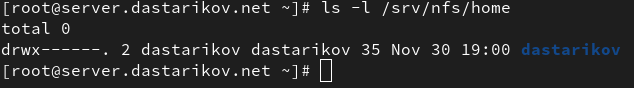
\includegraphics[width=\textwidth]{../images/image22.png}
    \captionof{figure}{Права каталога /srv/nfs/home/dastarikov.}
\end{frame}

\begin{frame}
\frametitle{Подключение каталогов для работы пользователей}
    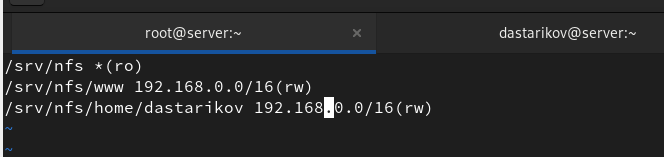
\includegraphics[width=\textwidth]{../images/image23.png}
    \captionof{figure}{Изменение файла /etc/exports.}
\end{frame}

\begin{frame}
\frametitle{Подключение каталогов для работы пользователей}
    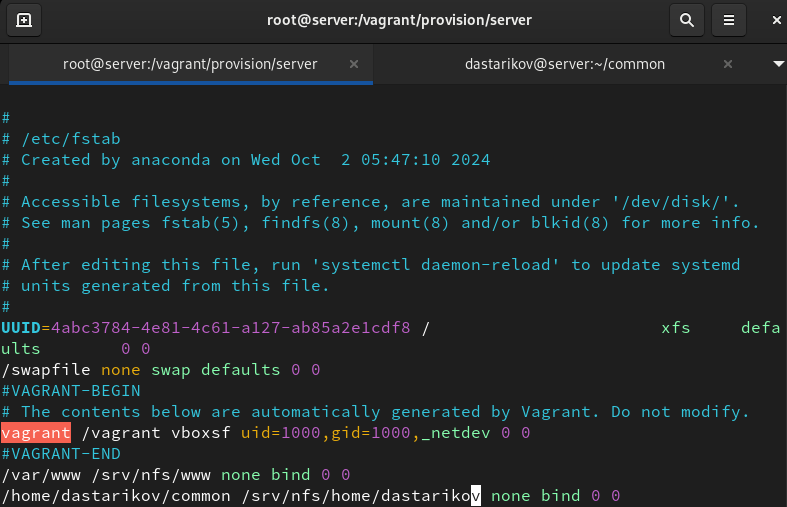
\includegraphics[width=\textwidth]{../images/image28.png}
    \captionof{figure}{Изменение /etc/fstab.}
\end{frame}

\begin{frame}
\frametitle{Подключение каталогов для работы пользователей}
    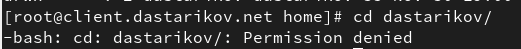
\includegraphics[width=\textwidth]{../images/image24.png}
    \captionof{figure}{Попытка зайти в каталог dastarikov на клиенте пользователем root.}
\end{frame}

\begin{frame}
\frametitle{Подключение каталогов для работы пользователей}
    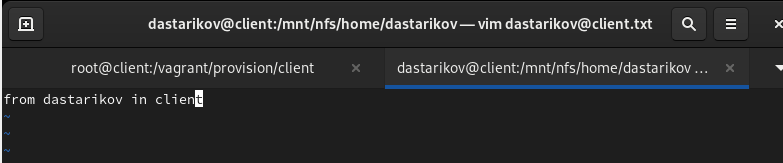
\includegraphics[width=\textwidth]{../images/image29.png}
    \captionof{figure}{Создание файла на клиенте.}
\end{frame}

\begin{frame}
\frametitle{Подключение каталогов для работы пользователей}
    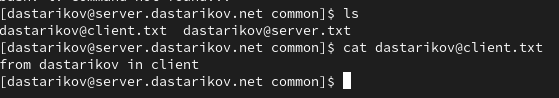
\includegraphics[width=\textwidth]{../images/image25.png}
    \captionof{figure}{Проверка изменений в локальном каталоге пользователя dastarikov.}
\end{frame}

% section 5

\begin{frame}
\frametitle{Внесение изменений в настройки внутреннего окружения виртуальных машин}
    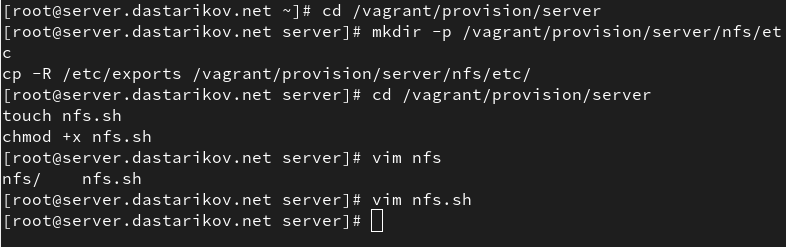
\includegraphics[width=\textwidth]{../images/image26.png}
    \captionof{figure}{Изменение настроек внутреннего окружения на виртуальной машине server.}
\end{frame}

\begin{frame}
\frametitle{Внесение изменений в настройки внутреннего окружения виртуальных машин}
    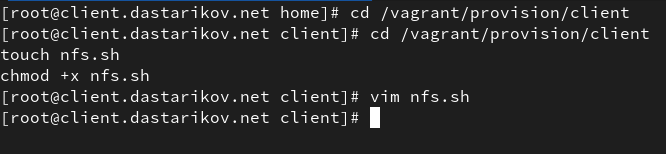
\includegraphics[width=\textwidth]{../images/image27.png}
    \captionof{figure}{Изменение настроек внутреннего окружения на виртуальной машине client.}
\end{frame}

\begin{frame}
\frametitle{Выводы}
\begin{itemize}
    \item В результате лабораторной работы познакомились с настройкой сервера NFS на примере создания каталога веб-сервера и каталога для удаленной работы конкретного пользователя.
\end{itemize}
\end{frame}
\end{document}
